\begin{infocard}{Proporcionalidad inversa}
    Colocaremos los 3 datos y la incógnita en la tabla igual que los hemos
    colocado en el caso anterior. Pero aplicaremos una fórmula distinta:
    \begin{center}
        \begin{tabular}{r>{\centering}p{0.2cm}l}
            $a$ & $\Rightarrow$ & $b$ \\
            $c$ & $\Rightarrow$ & $x$
        \end{tabular}\quad$x=\dfrac{a \times b}{c}$
    \end{center}
    % \begin{figure}[H]
    %     \centering
    %     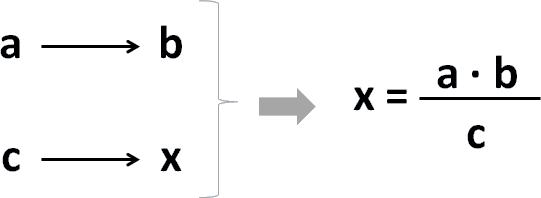
\includegraphics[width=.6\linewidth]{../images/formula-regla-de-3-img3}
    % \end{figure}
\end{infocard}